\section{Mechanism: Augmentation vs.\ Contrastive Objective}
\label{sec:mechanism}

To better understand the sources of SSL's tail-node benefit, we decompose the training pipeline into two components: (1) the regularizing effect of training on augmented graphs, and (2) the contrastive objective that enforces embedding invariance. We note that this decomposition is observational rather than causal; each component's contribution may depend on the other.

\paragraph{Decomposition experiment.}
We compare three training regimes: Vanilla (no augmentation), AugOnly (train on edge-dropped + noise-perturbed graph, no contrastive loss), and GlobalCL (augmentation + InfoNCE). Figure~\ref{fig:decomposition} shows cold-edge AUC gains over Vanilla.

\begin{figure}[t]
    \centering
    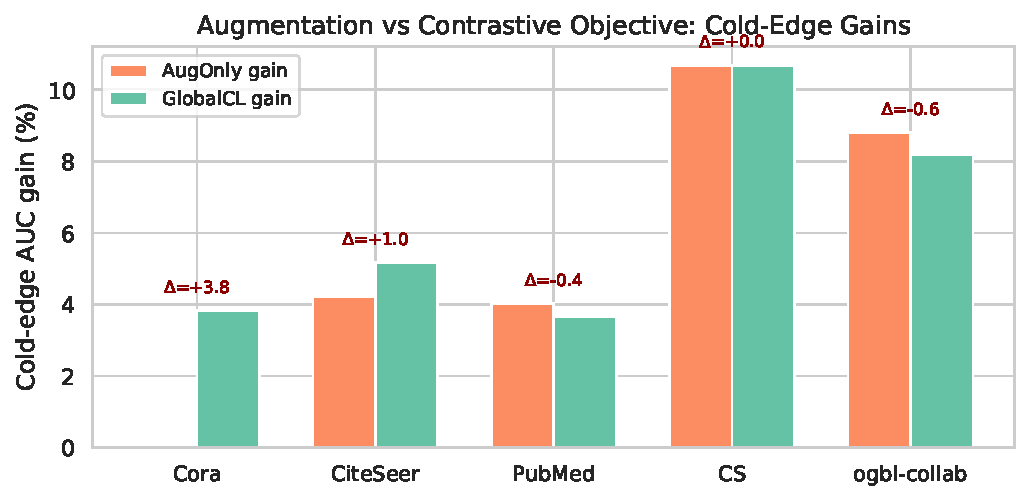
\includegraphics[width=\linewidth]{figures/fig3_decomposition.pdf}
    \caption{Decomposition of cold-edge gains. On small/sparse graphs (Cora), the contrastive objective adds substantial value (+2.4\%). On larger/denser graphs (CS, ogbl-collab), augmentation alone is sufficient.}
    \label{fig:decomposition}
\end{figure}

The results reveal a clear pattern tied to graph density:
\begin{itemize}[leftmargin=*, itemsep=2pt]
    \item \textbf{Cora} (small, sparse): AugOnly provides +1.5\% cold gain; GlobalCL adds +2.4\% more. The contrastive objective matters.
    \item \textbf{PubMed/CS} (medium, denser): AugOnly and GlobalCL provide similar cold gains (+4.0\% vs +3.6\% on PubMed). Augmentation dominates.
    \item \textbf{ogbl-collab} (large, dense): AugOnly (+8.8\%) \emph{outperforms} GlobalCL (+8.2\%). The contrastive objective adds no value.
\end{itemize}

\paragraph{Controlled sparsity experiment.}
To isolate the effect of graph density, we subsample edges from the CS and Cora training graphs at rates of 100\%, 75\%, 50\%, and 25\%, then compare AugOnly and GlobalCL at each sparsity level (Figure~\ref{fig:sparsity}).

\begin{figure}[t]
    \centering
    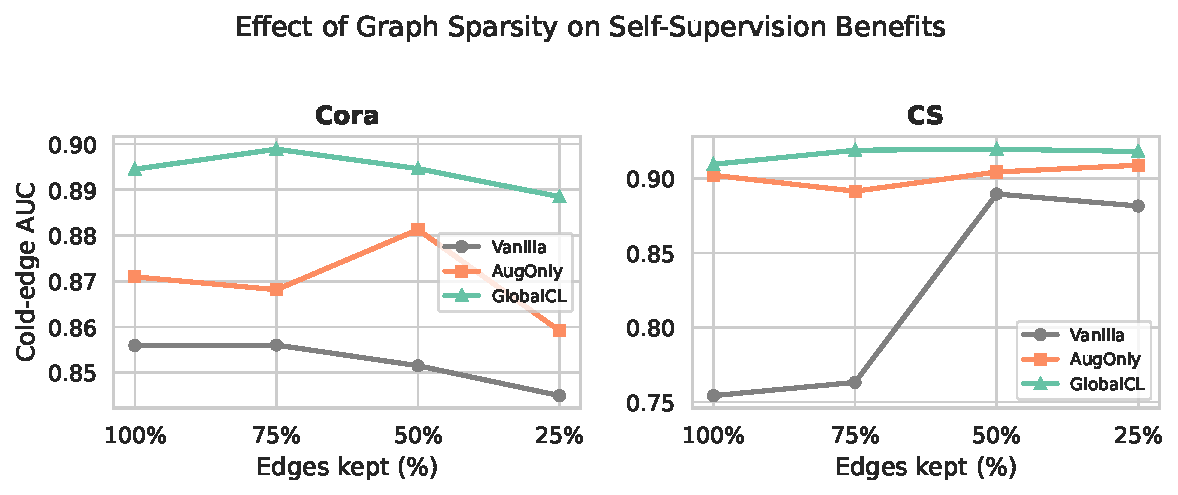
\includegraphics[width=\linewidth]{figures/fig5_sparsity.pdf}
    \caption{Cold-edge AUC under controlled sparsification. As graphs become sparser, all methods improve tail-node performance. The CL--AugOnly gap on Cora is consistently positive (+1--3\%), while on CS it is smaller.}
    \label{fig:sparsity}
\end{figure}

On Cora, GlobalCL maintains a consistent +1--3\% advantage over AugOnly across all sparsity levels, confirming that the contrastive objective provides value when structural context is limited. On CS, the gap is smaller and inconsistent, reflecting the sufficiency of augmentation regularization on denser graphs.

\paragraph{Interpretation.}
We hypothesize that augmentation acts as a structural regularizer, preventing GNNs from overfitting to the specific (sparse) neighborhood patterns of tail nodes. The contrastive objective provides additional value by enforcing embedding invariance across augmented views, which matters most when node neighborhoods are too small to provide stable representations through supervised training alone. On denser graphs, supervised aggregation already produces stable embeddings, making the contrastive invariance redundant.
